A Associação de Competições Maratonísticas (ACM) entrou em contato com a organização da Maratona Mineira de Programação para registrar uma reclamação:
por ter ``Maratona'' no nome, a competição estava recebendo muitas inscrições de corredores profissionais internacionais, em busca de pontos no
ranking mundial de corridas. Porém, no dia anterior à competição,
ao descobrirem que balões da Maratona Mineira não contam pontos no ranking da ACM, esses corredores se frustraram, retiraram
sua inscrição e voltaram para casa.
Para evitar esse mal entendido sem desperdiçar o potencial que a Maratona Mineira tem para cobrir outras modalidades,
a ACM e a organização da Mineira chegaram
a um acordo: a próxima edição da Mineira contará com uma corrida de 42km que somará pontos no ranking mundial da ACM!

Contudo, há um problema. Montar um bom circuito para uma Maratona é muito custoso, e a data da Mineira poderá colidir
com outros eventos na cidade. Sendo assim, a organização decidiu realizar a corrida em uma praça circular. Afinal, a distância que
pode ser percorrida dando voltas na praça é limitada apenas pela preparação do corredor!

Porém, pelas regras da ACM para minimizar lesões em corridas de longa distância, o circuito de corrida deve ser composto
unicamente por segmentos de reta.
As praças sendo consideradas pela organização possuem uma área interna, também circular, onde há um chafariz, e não é possível que o circuito
passe por aí. A praça tem raio $A$, e a área interna do chafariz tem raio $B$. Um circuito válido é um polígono que passa apenas pela área interna
da praça externa ao chafariz, e que contém a área do chafariz.

\begin{figure}[h]
\begin{center}
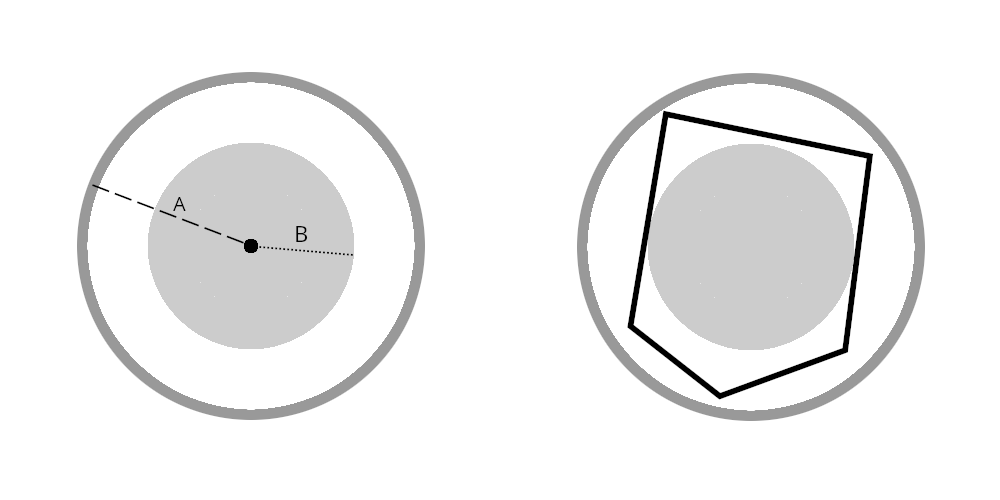
\includegraphics[height=15em]{\CWD/correndo}
\begin{quote}
\caption{Exemplo de praça com os raios $A$ e $B$ indicados, e um circuito possível composto de 5 segmentos de reta.}
\end{quote}
\end{center}
\end{figure}

A organização da Maratona Mineira está interessada em saber qual é o menor número de segmentos de reta necessários para se formar um circuito
válido em cada uma das praças que possivelmente serão escolhidas. Você pode ajudar?

\section*{Entrada}

A entrada contém apenas uma linha com dois inteiros $A$ e $B$, separados por espaço, representando os raios das circunferências interna e externa, respectivamente,
que formam a praça.

\section*{Saída}

Escreva na saída uma linha contendo um único inteiro $N$, o menor número de segmentos de reta necessários para formar um circuito válido na praça
dada.

\section*{Restrições}

$$1 \leq A < B \leq 10^9$$

\section*{Exemplos}
\exemplo
